\documentclass[preprint,12pt]{elsarticle}

\journal{Journal of Number Theory}

\usepackage[T1]{fontenc}
\usepackage[utf8]{inputenc}
\usepackage{lmodern}
\usepackage{amsmath,amssymb,amsfonts,amsthm,mathtools}
\usepackage{graphicx}
\usepackage[hidelinks]{hyperref}

\numberwithin{equation}{section}
\setcounter{secnumdepth}{3}
\emergencystretch=1.5em

\theoremstyle{plain}
\newtheorem{theorem}{Theorem}[section]
\newtheorem{proposition}[theorem]{Proposition}
\newtheorem{lemma}[theorem]{Lemma}
\newtheorem{corollary}[theorem]{Corollary}
\newtheorem{conjecture}[theorem]{Conjecture}

\theoremstyle{definition}
\newtheorem{experiment}[theorem]{Experiment}

\theoremstyle{remark}
\newtheorem{remark}[theorem]{Remark}

\begin{document}

\begin{frontmatter}

\title{Rational Resonances and Microscopic Natural--Logarithmic Profiles for the Liouville Function}

\author[uned]{Víctor Casaña-Giner\texorpdfstring{\corref{cor1}}{}}
\ead{vcasana1@alumno.uned.es}
\ead[url]{https://orcid.org/0000-0002-8252-2608}
\cortext[cor1]{Corresponding author.}
\affiliation[uned]{organization={Universidad Nacional de Educación a Distancia},
addressline={C/ Bravo Murillo, 38}, postcode={28015}, city={Madrid}, country={Spain}}

\begin{abstract}
Let $\lambda(n)=(-1)^{\Omega(n)}$ and
\[
C_X(u):=\sum_{\substack{1\le n\le X\\ \lfloor e^u n\rfloor\ge1}}
\lambda(n)\lambda(\lfloor e^u n\rfloor).
\]
For reduced rational dilations $e^u=p/q$, we isolate exactly the unique
proportional residue class. Assuming the standard fixed two-point affine
Chowla conjecture, this yields the natural microscopic profile
\[
\frac{1}{X}C_X\!\left(\log\frac pq+\frac cX\right)
\longrightarrow
\begin{cases}
0,&c<0,\\
\lambda(pq)/q,&0\le c\le q/p,\\
\lambda(pq)/(pc),&c>q/p.
\end{cases}
\]
The logarithmically weighted analogue has an unconditional one-sided
microscopic limit at the same $X^{-1}$ scale. At integer resonances we prove,
without Chowla input, a right-hand natural-average majority window
$0<c<2/m$ and a logarithmic mesoscopic majority theorem whose elementary
majority mechanism has threshold exponent $1/2$: every sequence
$c_X=X^{\theta+o(1)}$ with $\theta<1/2$ forces non-cancellation at the
corresponding right-hand scale $c_X/X=X^{-1+\theta+o(1)}$. Thus natural and logarithmic weighting exhibit different
microscopic scales, while integer resonances are singled out by unconditional
majority rigidity.
\end{abstract}

\begin{keyword}
Liouville function \sep Chowla conjecture \sep Beatty sequence \sep
rational resonance \sep logarithmic average \sep microscopic profile
\end{keyword}

\end{frontmatter}

\section{Introduction}
\label{sec:introduction}

The Liouville function $\lambda(n)=(-1)^{\Omega(n)}$ is completely
multiplicative. The fixed two-point Chowla conjecture predicts natural-average
cancellation of $\lambda$ on non-proportional affine forms. Tao proved the
corresponding logarithmically averaged two-point theorem
\cite{Tao2016}, while Matom\"aki--Radziwi{\l}{\l}--Tao proved an averaged
natural form \cite{MRT2015}. Arithmetic functions on Beatty sequences were
studied by Abercrombie \cite{Abercrombie1995} and
Abercrombie--Banks--Shparlinski \cite{AbercrombieBanksShparlinski2009}.

For irrational $\alpha$ with first slope equal to $1$, logarithmic
cancellation of
$\lambda(n)\lambda(\lfloor\alpha n\rfloor)$ was proved by
Crn\v{c}evi\'c, Hern\'andez, Rizk, Sereesuchart and R.~Tao
\cite{CHRST2024}. For a general irrational ratio of slopes, logarithmic
two-point cancellation is due to Ter\"av\"ainen and Walker
\cite[Theorem~1.2]{TeravainenWalker2025}; they moreover prove that in the
rationally dependent case the logarithmic limit exists and characterize when
it vanishes, answering the two-point case of a conjecture of Frantzikinakis
\cite{Frantzikinakis2020}. Neither cited theorem evaluates the non-vanishing
rational limit in closed form. The explicit value $\lambda(pq)/q$ used below
is obtained here from the residue-class decomposition together with Tao's
affine logarithmic cancellation. The new object is the singular
$X$-dependent perturbation
\[
u_X=\log(p/q)+c/X,
\]
together with its natural microscopic profile and the unconditional majority
phenomena that appear at integer resonances.

The structure is transparent. At a reduced rational dilation $p/q$, the
residue class $n\equiv0\pmod q$ is the unique proportional affine class; all
other residue classes are non-proportional. The natural main term is therefore
the sign $\lambda(pq)$ times the size of this proportional block, while the
remaining pieces require affine Chowla cancellation.

\section{Affine input and logarithmic normalization}
\label{sec:input}

\begin{conjecture}[Standard fixed two-point affine Chowla]
\label{conj:affine_chowla}
Let $a_1,a_2\in\mathbb N$ and $b_1,b_2\in\mathbb Z$ be fixed, with the two
affine forms positive for all sufficiently large $n$ and
$a_1b_2-a_2b_1\ne0$. Then
\[
\sum_{n\le Y}\lambda(a_1n+b_1)\lambda(a_2n+b_2)=o(Y).
\]
\end{conjecture}

No uniform or quantitative strengthening of this conjecture is used.

\begin{lemma}[Macroscopic subintervals]
\label{lem:macroscopic}
Assume Conjecture~\ref{conj:affine_chowla} for a fixed pair of affine forms.
If $A_X/X\to A$ and $B_X/X\to B$ with $0\le A\le B<\infty$, then the
corresponding sum over $A_X<n\le B_X$ is $o(X)$.
\end{lemma}

\begin{proof}
If $A<B$, subtract the two prefix estimates supplied by
Conjecture~\ref{conj:affine_chowla}. If $A=B$, the interval contains $o(X)$
integers and the trivial bound suffices.
\end{proof}

Let
\[
H_X:=\sum_{n\le X}\frac1n
\]
and define
\begin{equation}
C_X^{\log}(u):=
\frac1{H_X}
\sum_{\substack{1\le n\le X\\ \lfloor e^u n\rfloor\ge1}}
\frac{\lambda(n)\lambda(\lfloor e^u n\rfloor)}n.
\label{eq:logdef}
\end{equation}
Thus $|C_X^{\log}(u)|\le1$.

\begin{lemma}[Affine logarithmic cancellation with residue-class weight]
\label{lem:weighted_tao}
Let $A_1,A_2,Q\in\mathbb N$ and $B_1,B_2,A\in\mathbb Z$ be fixed.
Assume that the affine forms $A_1k+B_1$ and $A_2k+B_2$ are positive for all
sufficiently large $k$ and are non-proportional:
\begin{equation}
A_1B_2-A_2B_1\ne0.
\label{eq:weighted_tao_nonprop}
\end{equation}
If $Qk+A>0$ for all sufficiently large $k$, then
\begin{equation}
\sum_{\substack{k\le K\\A_1k+B_1\ge1\\A_2k+B_2\ge1}}
\frac{\lambda(A_1k+B_1)\lambda(A_2k+B_2)}{Qk+A}
=o(\log K).
\label{eq:weighted_tao}
\end{equation}
\end{lemma}

\begin{proof}
After deleting finitely many initial terms, and reindexing if necessary,
Tao's logarithmically averaged two-point theorem for fixed non-proportional
affine forms, specialized with $\omega(K)=K$, gives
\begin{equation}
\sum_{k\le K}
\frac{\lambda(A_1k+B_1)\lambda(A_2k+B_2)}{k}
=o(\log K).
\label{eq:tao_weight_one_over_k}
\end{equation}
The residue-class weight satisfies
\begin{equation}
\frac1{Qk+A}=\frac1Q\,\frac1k+O_{Q,A}(k^{-2}).
\label{eq:residue_weight_expansion}
\end{equation}
Since the Liouville product has modulus one, the total contribution of the
$O(k^{-2})$ error is $O(1)$. Combining
\eqref{eq:tao_weight_one_over_k} and
\eqref{eq:residue_weight_expansion} proves \eqref{eq:weighted_tao}.
\end{proof}

\section{Exact rational decomposition}
\label{sec:rational}

\begin{proposition}[Exact residue-class decomposition]
\label{prop:decomposition}
Let $(p,q)=1$ and $X\in\mathbb N$. Then
\begin{align}
C_X\!\left(\log\frac pq\right)
&=
\lambda(pq)\left\lfloor\frac Xq\right\rfloor \nonumber\\
&\quad+
\sum_{a=1}^{q-1}
\sum_{\substack{k\ge0\\1\le qk+a\le X\\
pk+\lfloor pa/q\rfloor\ge1}}
\lambda(qk+a)
\lambda\!\left(pk+\left\lfloor\frac{pa}{q}\right\rfloor\right).
\label{eq:decomp}
\end{align}
For every $a\ne0$ the two affine forms in the inner sum are
non-proportional.
\end{proposition}

\begin{proof}
Write $n=qk+a$, $0\le a<q$. Then
\[
\left\lfloor\frac pq(qk+a)\right\rfloor
=
pk+\left\lfloor\frac{pa}{q}\right\rfloor.
\]
For $a=0$ and $k\ge1$, complete multiplicativity gives
$\lambda(qk)\lambda(pk)=\lambda(pq)$. For $a\ne0$, proportionality would
require $q\lfloor pa/q\rfloor=pa$, impossible because $(p,q)=1$ and
$q\nmid a$.
\end{proof}

\begin{theorem}[Fixed rational natural resonance]
\label{thm:fixed}
Assume Conjecture~\ref{conj:affine_chowla}. Then
\[
\frac1X C_X\!\left(\log\frac pq\right)\longrightarrow\frac{\lambda(pq)}q.
\]
For $q=1$ the exact identity
\[
C_X(\log p)=\lambda(p)X
\]
holds for every $X\in\mathbb N$.
\end{theorem}

\begin{proof}
The proportional class in Proposition~\ref{prop:decomposition} contributes
$\lambda(pq)\lfloor X/q\rfloor$. Every other residue class is a fixed
non-proportional affine correlation and is $o(X)$ by
Conjecture~\ref{conj:affine_chowla}. For $q=1$ there are no remaining
classes.
\end{proof}

\section{Unconditional logarithmic microscopic step}
\label{sec:logstep}

\begin{theorem}[Logarithmic microscopic step]
\label{thm:logstep}
Let $(p,q)=1$ and let $c\in\mathbb R$ be fixed. Then
\begin{equation}
C_X^{\log}\!\left(\log\frac pq+\frac cX\right)
\longrightarrow
\frac{\lambda(pq)}q\,\mathbf 1_{\{c\ge0\}}
\label{eq:logstep}
\end{equation}
unconditionally.
\end{theorem}

\begin{proof}
Fix $\varepsilon\in(0,1)$ and set
\begin{equation}
Y=X^{1-\varepsilon}.
\label{eq:logstep_Y}
\end{equation}
Write $n=qk+a$, $0\le a<q$. Uniformly for $n\le Y$,
\begin{equation}
\frac pq(e^{c/X}-1)n=O_{p,q,c}(X^{-\varepsilon}).
\label{eq:logstep_small_perturbation}
\end{equation}
If $a=0$, then $\{pa/q\}=0$. When $q=1$ there are no nonzero residue classes. If $a\ne0$, coprimality gives
\begin{equation}
\left\{\frac{pa}{q}\right\}\in
\left[\frac1q,1-\frac1q\right].
\label{eq:logstep_fractional_separation}
\end{equation}
Hence, for all sufficiently large $X$, the perturbation in
\eqref{eq:logstep_small_perturbation} cannot change the floor on any
$a\ne0$ residue class.

Suppose first that $c\ge0$. On $n\le Y$ the perturbed correlation agrees
exactly with the fixed rational dilation. The proportional class $a=0$
contributes
\begin{equation}
\frac{\lambda(pq)}{H_X}
\sum_{k\le Y/q}\frac1{qk}
=
\frac{H_Y}{H_X}\frac{\lambda(pq)}q+o(1).
\label{eq:logstep_prop_initial}
\end{equation}
For each $a\ne0$, the two fixed affine forms are non-proportional, so
Lemma~\ref{lem:weighted_tao}, with weight $(qk+a)^{-1}$, shows that its
entire contribution on $n\le Y$ is $o(H_Y)$ and therefore $o(1)$ after
division by $H_X$. The tail $Y<n\le X$ has normalized harmonic mass
\begin{equation}
\frac{H_X-H_Y}{H_X}=\varepsilon+o(1).
\label{eq:logstep_tail_mass}
\end{equation}
Consequently,
\begin{equation}
\left|
C_X^{\log}\!\left(\log\frac pq+\frac cX\right)
-\frac{H_Y}{H_X}\frac{\lambda(pq)}q
\right|
\le
\frac{H_X-H_Y}{H_X}+o(1).
\label{eq:logstep_bilateral}
\end{equation}
Since $H_Y/H_X\to1-\varepsilon$, first letting $X\to\infty$ and then
$\varepsilon\downarrow0$ gives the branch $c\ge0$. This derivation makes the
explicit value $\lambda(pq)/q$ independent of any stronger reading of the
rational case of Ter\"av\"ainen--Walker. Their framework is consistent with,
and also yields, the rationally dependent non-zero alternative
\cite[Theorem~1.2(3)]{TeravainenWalker2025}.

Now suppose that $c<0$. On the class $a=0$ and the range $n=qk\le Y$,
\eqref{eq:logstep_small_perturbation} gives
\begin{equation}
\left\lfloor pe^{c/X}k\right\rfloor=pk-1
\label{eq:logstep_negative_zero_class}
\end{equation}
for every $k\ge1$ once $X$ is large, except for the possible initial term
for which the target equals zero and is excluded by definition. To apply
Tao in the usual non-negative-intercept formulation, write $k=\ell+1$:
\begin{equation}
qk=q\ell+q,\qquad pk-1=p\ell+(p-1).
\label{eq:logstep_reindex}
\end{equation}
If $p=1$, the single term with second value zero is omitted; the remaining
terms may be reindexed once more. The two forms are non-proportional. Every
$a\ne0$ class remains non-proportional by
\eqref{eq:logstep_fractional_separation}. Lemma~\ref{lem:weighted_tao}
therefore makes the whole initial range $o(H_Y)$, while the tail is bounded
by \eqref{eq:logstep_tail_mass}. Letting $X\to\infty$ and then
$\varepsilon\downarrow0$ gives zero.
\end{proof}

\section{Conditional natural microscopic profile}
\label{sec:natural}

\begin{theorem}[Rational natural microscopic profile]
\label{thm:profile}
Assume Conjecture~\ref{conj:affine_chowla}.\par
Let $(p,q)=1$ and fix $c\in\mathbb R$. Then
\begin{equation}
\frac1X C_X\!\left(\log\frac pq+\frac cX\right)
\longrightarrow
\Psi_{p,q}(c),
\label{eq:profilelimit}
\end{equation}
where
\begin{equation}
\Psi_{p,q}(c)=
\begin{cases}
0,&c<0,\\[1mm]
\dfrac{\lambda(pq)}q,&0\le c\le q/p,\\[3mm]
\dfrac{\lambda(pq)}{pc},&c>q/p.
\end{cases}
\label{eq:profile}
\end{equation}
For $c>0$,
\[
\Psi_{p,q}(c)=
\lambda(pq)\min\!\left(\frac1q,\frac1{pc}\right).
\]
\end{theorem}

\begin{proof}
Put
\[
\delta_X:=\frac pq(e^{c/X}-1)
\]
and write $n=qk+a$, $0\le a<q$. Then
\begin{equation}
\left\lfloor e^{\log(p/q)+c/X}(qk+a)\right\rfloor
=
pk+
\left\lfloor\frac{pa}{q}+\delta_X(qk+a)\right\rfloor.
\label{eq:perturbedfloor}
\end{equation}

Assume first $c>0$. For an integer $r$, the block on which the final floor in
\eqref{eq:perturbedfloor} equals $\lfloor pa/q\rfloor+r$ is
\[
r\le
\left\{\frac{pa}{q}\right\}+\delta_X(qk+a)<r+1.
\]
Equivalently,
\begin{align}
\frac{r-\{pa/q\}}{Xp(e^{c/X}-1)}
-\frac{a}{qX}
\le \frac{k}{X}
<
\frac{r+1-\{pa/q\}}{Xp(e^{c/X}-1)}
-\frac{a}{qX}.
\label{eq:blockinterval}
\end{align}
Since $Xp(e^{c/X}-1)\to pc$, both endpoints converge. After intersection
with $0\le k/X\le1/q+O(X^{-1})$, each block has endpoints converging to
fixed limits. If the limiting endpoints are distinct, the block is
macroscopic; if they coincide, its length is $o(X)$; otherwise it is empty.
For fixed $p,q,c$, the perturbation in \eqref{eq:perturbedfloor} is uniformly
bounded for $0\le n\le X$, so the number of integers $r$ that occur is
bounded in terms of $p,q,c$ and is independent of $X$.

On such a block the two affine forms are
\[
qk+a,\qquad
pk+\left\lfloor\frac{pa}{q}\right\rfloor+r.
\]
For $a\ne0$, proportionality would require
\[
qr=pa-q\left\lfloor\frac{pa}{q}\right\rfloor
=pa\bmod q\in\{1,\ldots,q-1\},
\]
which is impossible. For $a=0$, proportionality occurs only for $r=0$.
Thus every block except $(a,r)=(0,0)$ is $o(X)$ by
Lemma~\ref{lem:macroscopic}.

The unique proportional block is
\[
n=qk,\qquad p(e^{c/X}-1)k<1.
\]
Its cardinality is
\[
R_X(c)=
\min\!\left(
\left\lfloor\frac Xq\right\rfloor,
\left\lceil\frac1{p(e^{c/X}-1)}\right\rceil-1
\right),
\]
up to the harmless endpoint convention. Hence
\[
\frac{R_X(c)}X\longrightarrow
\min\!\left(\frac1q,\frac1{pc}\right),
\]
and every term in this block equals $\lambda(pq)$.

If $c<0$, the same block decomposition has negative corrections. For
$a=0$ the correction is a nonzero negative integer for every $k\ge1$, so no
proportional block remains. For $a\ne0$, proportionality would again imply
$qr=pa\bmod q$, impossible. Only finitely many negative correction integers occur for fixed $p,q,c$.
For each such correction, the target affine form can fail to be positive only
for $O_{p,q,c}(1)$ initial values of $k$; these terms are omitted by the
definition of $C_X$. All remaining blocks are $o(X)$.

At $c=0$, Theorem~\ref{thm:fixed} applies. At the boundary $pc=q$,
\[
\frac{pX}{q}(e^{c/X}-1)
=
1+\frac{q}{2pX}+O(X^{-2}),
\]
so only $O(1)$ terminal terms leave the proportional block. The normalized
limit remains $\lambda(pq)/q$.
\end{proof}

\section{Integer rigidity and unconditional majority}
\label{sec:integer}

\begin{corollary}[Integer profile and exact right-hand plateau]
\label{cor:integer}
Assume Conjecture~\ref{conj:affine_chowla}. For fixed $m\ge2$,
\[
\frac1X C_X\!\left(\log m+\frac cX\right)
\longrightarrow
\begin{cases}
0,&c<0,\\
\lambda(m),&0\le c\le1/m,\\
\lambda(m)/(mc),&c>1/m.
\end{cases}
\]
Moreover, for every fixed $0<c<1/m$,
\[
C_X\!\left(\log m+\frac cX\right)=\lambda(m)X
\]
for all sufficiently large $X$.
\end{corollary}

\begin{proof}
The limit is Theorem~\ref{thm:profile} with $q=1$. For the exact statement,
$mX(e^{c/X}-1)\to mc<1$, so eventually no correction occurs for any
$n\le X$.
\end{proof}

\begin{theorem}[Unconditional right-hand natural majority window]
\label{thm:naturalmajority}
Let $m\ge2$ and $0<c<2/m$. Then
\begin{equation}
\liminf_{X\to\infty}
\lambda(m)\frac1X
C_X\!\left(\log m+\frac cX\right)
\ge
2\min\!\left(1,\frac1{mc}\right)-1>0.
\label{eq:naturalmajority}
\end{equation}
\end{theorem}

\begin{proof}
Let
\[
I_{0,X}:=\{1\le n\le X:m(e^{c/X}-1)n<1\}.
\]
Every summand on $I_{0,X}$ equals $\lambda(m)$, while every remaining term
has modulus at most one. Therefore
\[
\lambda(m)C_X\!\left(\log m+\frac cX\right)\ge2|I_{0,X}|-X.
\]
Since
\[
\frac{|I_{0,X}|}{X}\to\min\!\left(1,\frac1{mc}\right),
\]
the result follows. This is a signed lower bound; absolute
non-cancellation follows immediately.
\end{proof}

\begin{theorem}[Unconditional logarithmic mesoscopic majority]
\label{thm:logmajority}
Let $(p,q)=1$ and let $c_X>0$ satisfy
\[
\frac{\log c_X}{\log X}\longrightarrow\theta,
\qquad 0\le\theta<1.
\]
Then
\begin{equation}
\liminf_{X\to\infty}
\lambda(pq)\,
C_X^{\log}\!\left(\log\frac pq+\frac{c_X}{X}\right)
\ge
\frac{2(1-\theta)}q-1.
\label{eq:logmajority}
\end{equation}
In particular, when $q=1$ and $\theta<1/2$,
\[
\liminf_{X\to\infty}
\lambda(m)C_X^{\log}\!\left(\log m+\frac{c_X}{X}\right)
\ge1-2\theta>0.
\]
Thus $1/2$ is the threshold exponent for this elementary logarithmic
majority mechanism. More precisely, for every sequence
$c_X=X^{\theta+o(1)}$ with $\theta<1/2$, it forces non-cancellation at the
right-hand displacement $c_X/X=X^{-1+\theta+o(1)}$; in particular this
includes $X^{-1/2-\varepsilon+o(1)}$ for every $\varepsilon>0$.
For $q\ge2$, the same trivial majority bound yields no positive lower bound.
\end{theorem}

\begin{proof}
On the proportional class $n=qk$, the zero-correction condition is
\[
p(e^{c_X/X}-1)k<1.
\]
Let $K_X$ be the largest admissible $k$, truncated by $k\le X/q$. Since
$c_X=X^{\theta+o(1)}$ and $\theta<1$,
\[
K_X=X^{1-\theta+o(1)}.
\]
The normalized harmonic mass of this block is
\[
B_X=
\frac1{H_X}\sum_{k\le K_X}\frac1{qk}
=
\frac{1-\theta}{q}+o(1).
\]
After multiplication by $\lambda(pq)$, all terms on this block are positive.
The complement has total normalized harmonic mass at most $1-B_X$, so
\[
\lambda(pq)C_X^{\log}\ge B_X-(1-B_X)=2B_X-1.
\]
This proves \eqref{eq:logmajority}. For $q=1$, positivity is equivalent to
$\theta<1/2$. Taking $c_X=X^{1/2-\varepsilon}$ gives the displacement
$c_X/X=X^{-1/2-\varepsilon}$.
\end{proof}

\begin{remark}[Positive fixed logarithmic branch from the majority theorem]
For $q=1$ and $\theta=0$, Theorem~\ref{thm:logmajority} gives
$\liminf\lambda(m)C_X^{\log}\ge1$, while $|C_X^{\log}|\le1$. Hence
\[
C_X^{\log}\!\left(\log m+\frac{c_X}{X}\right)\to\lambda(m)
\]
for every positive $c_X$ with $\log c_X/\log X\to0$. No logarithmic Chowla
input is needed for this integer positive branch.
\end{remark}

\begin{remark}[The endpoint $c=1/m$ is not an exact finite plateau]
For the integer right-hand layer,
\[
Xm(e^{1/(mX)}-1)
=
1+\frac1{2mX}+O(X^{-2})>1.
\]
Thus $c=1/m$ belongs to the closed limiting plateau but not to the eventual
exact finite plateau. For $m=2$, $X=10^6$, the regenerated computation gives
$C_X=-999998$.
\end{remark}

\begin{proposition}[Exact left-hand $c$-independence interval]
\label{prop:left}
Let $m\ge2$ and fix $-1/m<c<0$. For all sufficiently large $X$,
\[
C_X\!\left(\log m+\frac cX\right)
=
\sum_{n\le X}\lambda(n)\lambda(mn-1).
\]
This states exact independence with respect to $c$ on that finite interval;
no asymptotic value of the right-hand sum is asserted.
\end{proposition}

\begin{proof}
Put $\beta_X=m(1-e^{c/X})$. Since $X\beta_X\to m|c|<1$, eventually
$0<\beta_Xn<1$ for all $n\le X$. Hence
$\lceil\beta_Xn\rceil=1$ and $\lfloor me^{c/X}n\rfloor=mn-1$.
\end{proof}

\begin{proposition}[Locally finite step structure]
Fix $m\ge2$ and $X\in\mathbb N$. The map
\[
c\longmapsto C_X\!\left(\log m+\frac cX\right)
\]
is locally constant except at explicit crossing values. Every compact
$c$-interval contains only finitely many jumps. For sufficiently negative
$c$, disappearance points where $\lfloor me^{c/X}n\rfloor<1$ are included
among these crossings.
\end{proposition}

\begin{proof}
For each fixed $n\le X$, the integer $\lfloor me^{c/X}n\rfloor$ changes only
when the continuous function $me^{c/X}n$ crosses an integer. On a compact
$c$-interval its range is bounded, hence only finitely many crossings occur.
There are only finitely many $n\le X$.
\end{proof}

\section{Numerical verification}
\label{sec:numerics}

All values below were regenerated from the supplied signed-int8 Liouville
prefix using the supplied Python scripts. They are finite checks and are not
used as asymptotic rate assumptions.

\begin{experiment}[Fixed rational resonances]
At $X=2\cdot10^6$:
\[
\begin{array}{c|r|r|r}
p/q & C_X/X & \lambda(pq)/q & (C_X-X\lambda(pq)/q)/\sqrt X\\ \hline
3/2 &  0.4999230 &  0.5000000 & -0.109\\
5/2 &  0.4995180 &  0.5000000 & -0.682\\
7/2 &  0.4996260 &  0.5000000 & -0.529\\
2/3 &  0.3326445 &  0.3333333 & -0.974\\
5/3 &  0.3324220 &  0.3333333 & -1.289\\
4/3 & -0.3322400 & -0.3333333 &  1.546\\
5/4 & -0.2492080 & -0.2500000 &  1.120
\end{array}
\]
The $2/3$ computation omits the unique initial term for which
$\lfloor(2/3)n\rfloor=0$, as required by the definition.
\end{experiment}

\begin{figure}[htbp]
\centering
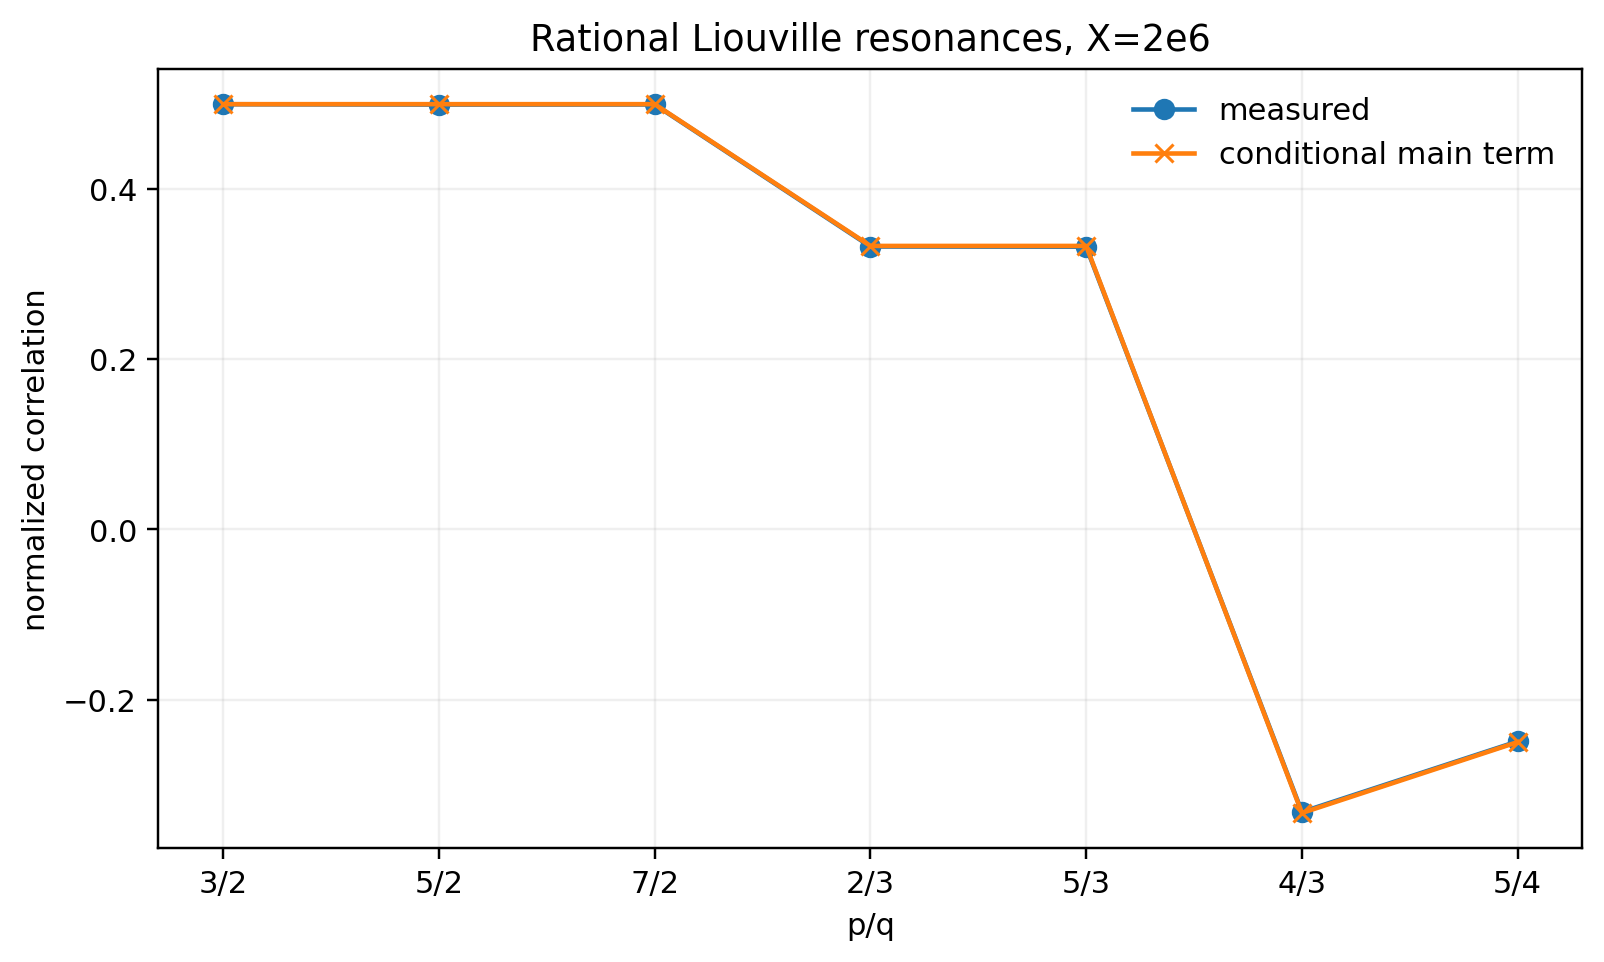
\includegraphics[width=.88\textwidth]{rational_resonances_X2000000.png}
\caption{Measured rational resonances at $X=2\cdot10^6$ and the conditional
natural main term.}
\label{fig:rational}
\end{figure}

\begin{experiment}[Natural microscopic profile]
For $p/q=3/2$ and $X=2\cdot10^6$:
\[
\begin{array}{c|r|r}
c & C_X/X & \Psi_{3,2}(c)\\ \hline
-0.5 & -0.000265 & 0\\
-0.1 & -0.000321 & 0\\
0.0 & 0.499923 & 0.500000\\
0.3 & 0.499923 & 0.500000\\
0.6 & 0.499904 & 0.500000\\
0.8 & 0.415884 & 0.416667\\
1.2 & 0.276538 & 0.277778\\
2.0 & 0.166553 & 0.166667
\end{array}
\]
\end{experiment}

\begin{figure}[htbp]
\centering
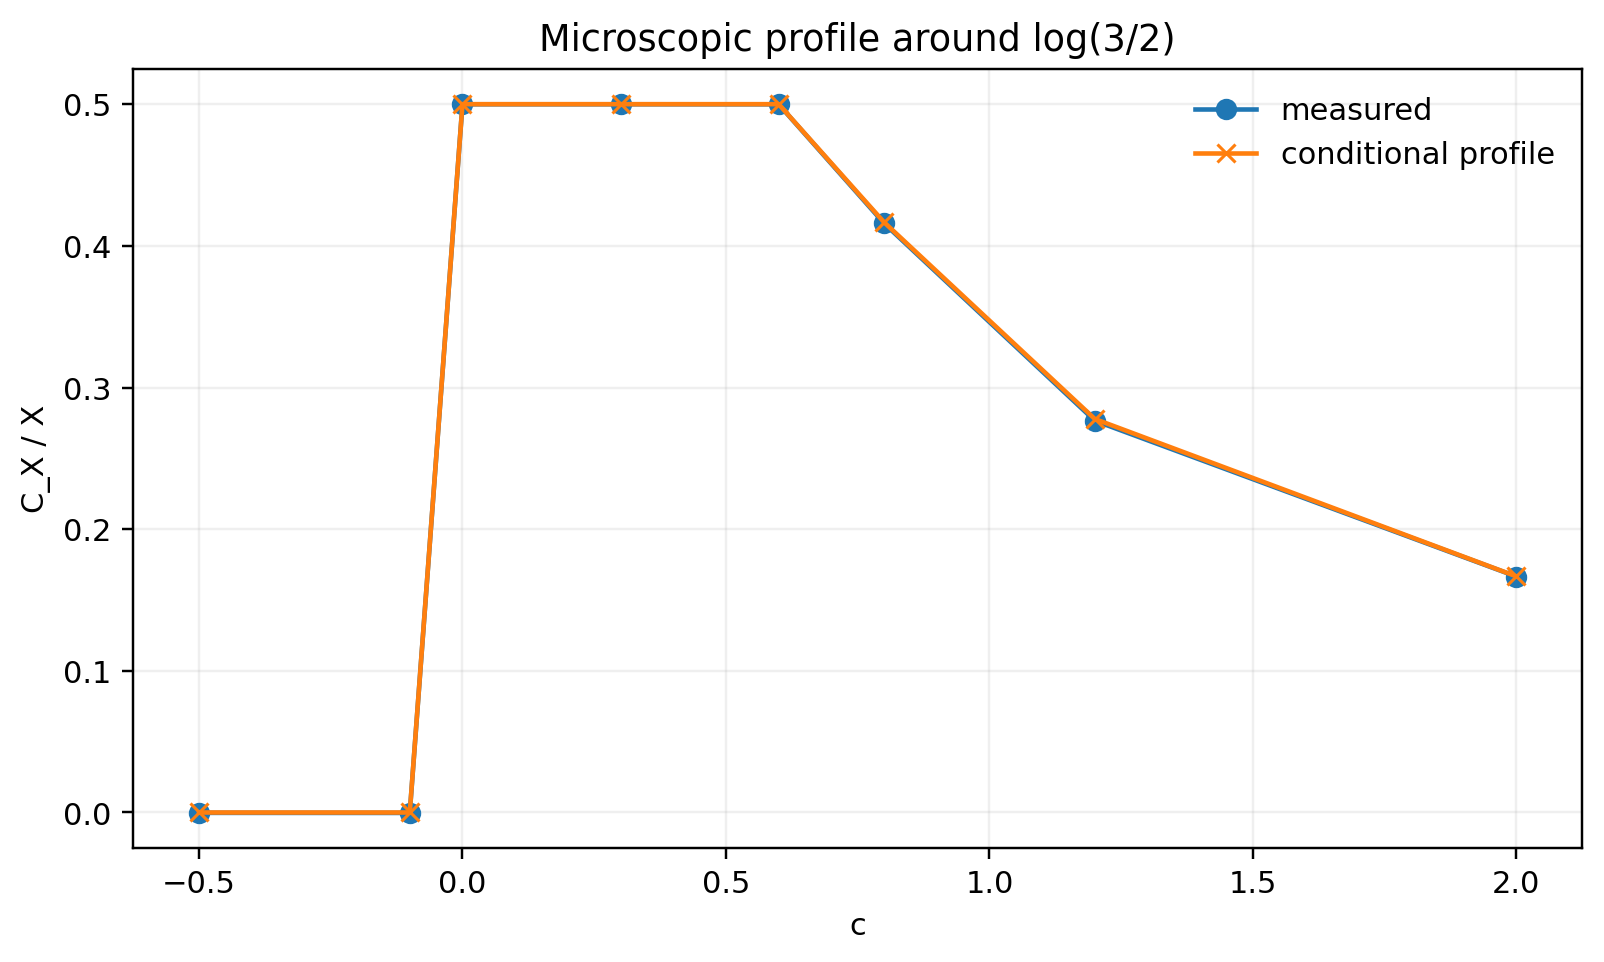
\includegraphics[width=.88\textwidth]{rational_local_profile_3_over_2.png}
\caption{Natural microscopic profile around $\log(3/2)$.}
\label{fig:profile}
\end{figure}

\begin{experiment}[Integer endpoint, left interval, and majority]
For $m=2$, $X=10^6$, $c=1/2$,
\[
Xm(e^{c/X}-1)=1.000000250000041666\ldots,\qquad C_X=-999998.
\]
For $m=2$, $X=10^7$, both $c=-0.01$ and $c=-0.40$ give exactly
$C_X=-778$. The complete finite verification of
Theorem~\ref{thm:naturalmajority} is supplied in the output files.
\end{experiment}

\begin{experiment}[Logarithmic mesoscopic majority]
For $m=2$, $X=10^7$ and $c_X=X^\theta$, the supplied script evaluates
$C_X^{\log}$, the exact resonant harmonic mass, and the bound in
Theorem~\ref{thm:logmajority}. The values are included in the supplementary
CSV and text outputs.
\end{experiment}

\begin{figure}[htbp]
\centering
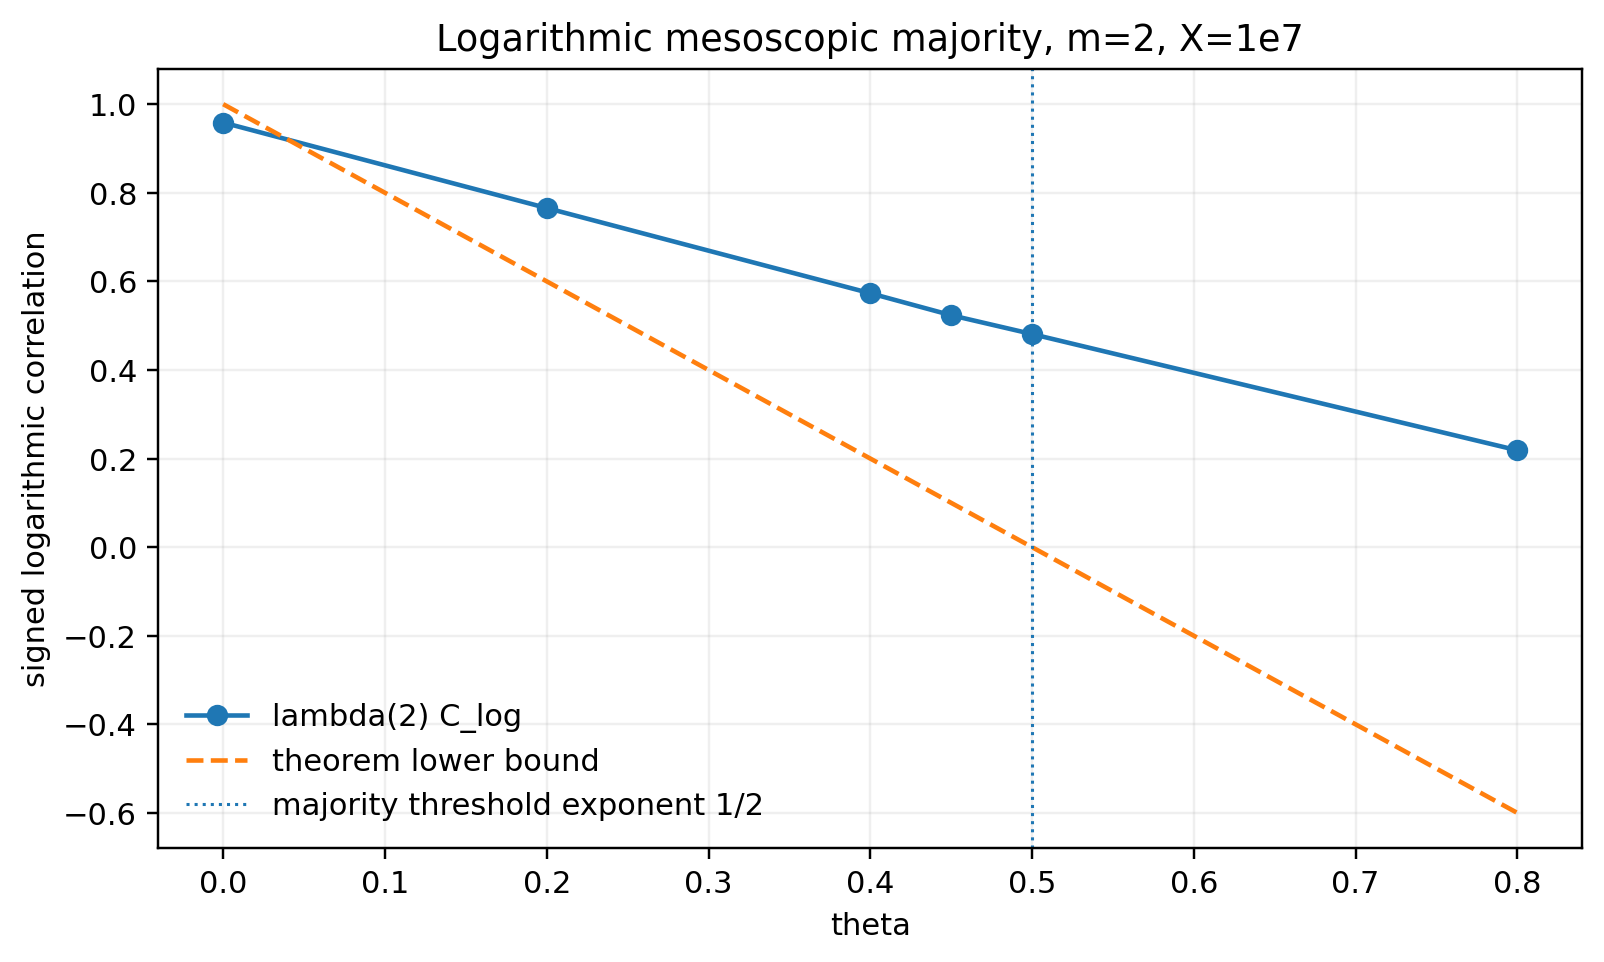
\includegraphics[width=.88\textwidth]{logarithmic_mesoscopic_m2_X10000000.png}
\caption{Finite logarithmic mesoscopic check for $m=2$, $X=10^7$. The dashed
curve is the envelope supplied by the unconditional signed majority bound.}
\label{fig:logmajority}
\end{figure}

\section{Conclusions}
\label{sec:conclusions}

Reduced rational dilations decompose into one proportional residue class and
finitely many non-proportional affine classes. Under fixed affine Chowla this
produces the natural microscopic profile
$\lambda(pq)\min(1/q,1/(pc))$ on the positive side and zero on the negative
side. Logarithmic weighting behaves differently: the fixed $X^{-1}$ layer
collapses to a one-sided step, while the elementary logarithmic majority mechanism has threshold
exponent $1/2$ and is effective for every
$c_X=X^{\theta+o(1)}$ with $\theta<1/2$. These unconditional majority
statements distinguish integer from non-integer rational resonances without
using Chowla, while the conditional and unconditional parts of the argument
remain separated explicitly throughout.

\section{Data and reproducibility}
\label{sec:data}

The numerical calculations use only
\path{liouville_int8_N21000000.bin}, containing the first $21{,}000{,}000$
Liouville values as signed int8 with byte $n-1$ equal to $\lambda(n)$. The
binary is deterministically reproducible from
$\lambda(n)=(-1)^{\Omega(n)}$ using the supplied generator. The repository
contains every Python script used for the reported checks, all corresponding
stdout captures, CSV and text outputs, the three manuscript figures as PNG
files, and SHA-256 inventories for the submission files and the complete
repository.

\section{Use of AI tools}
\label{sec:ai}

AI tools were used during drafting, code development, and consistency
checking. All mathematical claims retained in the manuscript were reviewed by
the author. All reported numerical values were regenerated from the supplied
Liouville binary by the supplied Python scripts and checked against the
identities stated in the manuscript. The author verified the resulting
computations and remains responsible for the manuscript and its numerical
content.

\begin{thebibliography}{99}
\raggedright

\bibitem{Abercrombie1995}
A.~G. Abercrombie,
\textit{Beatty sequences and multiplicative number theory},
Acta Arith. 70 (1995), 195--207; DOI: \nolinkurl{10.4064/aa-70-3-195-207}.

\bibitem{AbercrombieBanksShparlinski2009}
A.~G. Abercrombie, W.~D. Banks, I.~E. Shparlinski,
\textit{Arithmetic functions on Beatty sequences},
Acta Arith. 136 (2009), 81--89; DOI: \nolinkurl{10.4064/aa136-1-6}.

\bibitem{Frantzikinakis2020}
N. Frantzikinakis,
\textit{Correlations of multiplicative functions along deterministic and
independent sequences},
arXiv:1908.02732.

\bibitem{CHRST2024}
D. Crn\v{c}evi\'c, F. Hern\'andez, K. Rizk, K. Sereesuchart, R. Tao,
\textit{On the multiplicative independence between $n$ and
$\lfloor \alpha n\rfloor$},
Acta Arith. 213 (2024), 193--226;
DOI: \nolinkurl{10.4064/aa230115-18-2};
arXiv:2211.15830.

\bibitem{MRT2015}
K. Matom\"aki, M. Radziwi{\l}{\l}, T. Tao,
\textit{An averaged form of Chowla's conjecture},
Algebra Number Theory 9 (2015), 2167--2196; DOI: \nolinkurl{10.2140/ant.2015.9.2167}.

\bibitem{Tao2016}
T. Tao,
\textit{The logarithmically averaged Chowla and Elliott conjectures for
two-point correlations},
Forum Math. Pi 4 (2016), e8; DOI: \nolinkurl{10.1017/fmp.2016.6};
arXiv:1509.05422.

\bibitem{TeravainenWalker2025}
J. Ter\"av\"ainen, A. Walker,
\textit{On a Bohr set analogue of Chowla's conjecture},
Math. Z. 310 (2025), Article 75; DOI: \nolinkurl{10.1007/s00209-025-03770-2};
arXiv:2303.12574.

\end{thebibliography}

\end{document}
